\section{Schaffer Function N.2}
  The \emph{Schaffer Function N.2} is a well-established mathematical function
  frequently used in the realm of algorithm testing.
  It serves as a performance benchmark for a wide array of optimization
  algorithms, particularly those grounded in evolutionary computation and swarm 
  intelligence principles.

  \begin{definition}[Schaffer Function N.2]
    The Schaffer Function N.2 is defined over a two-dimensional domain, mapping 
    \(\mathbb{R}^2\) to \(\mathbb{R}\).
    The function, denoted as \(f(\mathbf{x})\), is expressed as follows:

    \[
      f(\mathbf{x}) = 0.5 + \frac{
          \sin^2(\sqrt{x_1^2 + x_2^2}) - 0.5
        }{
          (1.0 + 0.001 \cdot (x_1^2 + x_2^2))^2
        }
    \]

    Here, \(\mathbf{x} = (x_1, x_2)\) represents a point in the two-dimensional
     domain, with \(x_1, x_2\) each ranging within the interval [-100, 100].
  \end{definition}

  The Schaffer Function N.2 achieves its global minimum at \(f(0,\,0) = 0\).
  A visual exploration of this function can be enhanced by both contour and 
  surface plots, providing a clearer understanding of its global minimum and 
  topological characteristics.
  Refer to \vref{fig:app:test:schaffer_2} for the corresponding plots.

  \begin{figure}[ht!]
    \centering
    \begin{subfigure}[b]{0.45\textwidth}
      \centering
      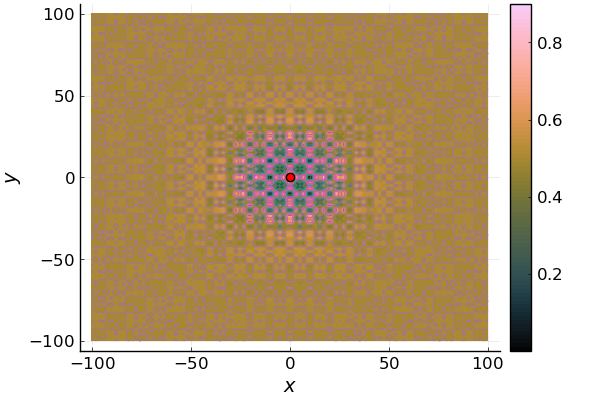
\includegraphics[width=\textwidth]
        {img/test_functions/schaffer_2_contour.png}
      \caption{Contour plot of the Schaffer Function N.2}
    \end{subfigure}
    \hfill
    \begin{subfigure}[b]{0.45\textwidth}
      \centering
      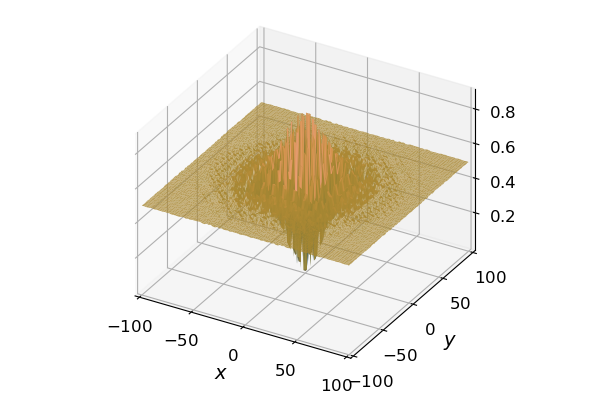
\includegraphics[width=\textwidth]
        {img/test_functions/schaffer_2_surface.png}
      \caption{Surface plot of the Schaffer Function N.2}
    \end{subfigure}
    \caption{
      Visualization of the Schaffer Function N.2.
      The contour and surface plots illustrate the function's topology, with the
      global minimum denoted by a red dot.
    }
    \label{fig:app:test:schaffer_2}
  \end{figure}
